
This chapter describes the experimental setup used to evaluate the modular RollupX ZK-rollup prototype. The evaluation is designed as a controlled benchmark study, where selected configuration variables are changed while the rest of the environment is kept stable. This allows the experiments to isolate how batching, sequencing, proving, data availability, and workload settings affect throughput, latency, finalization time, and cost.

Before presenting the individual benchmark scenarios, Figure~\ref{fig:experiment_matrix_structure} summarizes the overall experiment matrix. The matrix groups the evaluation dimensions into configurable system variables, workload variables, and observed performance metrics.

\begin{figure}[!htbp]
    \centering
    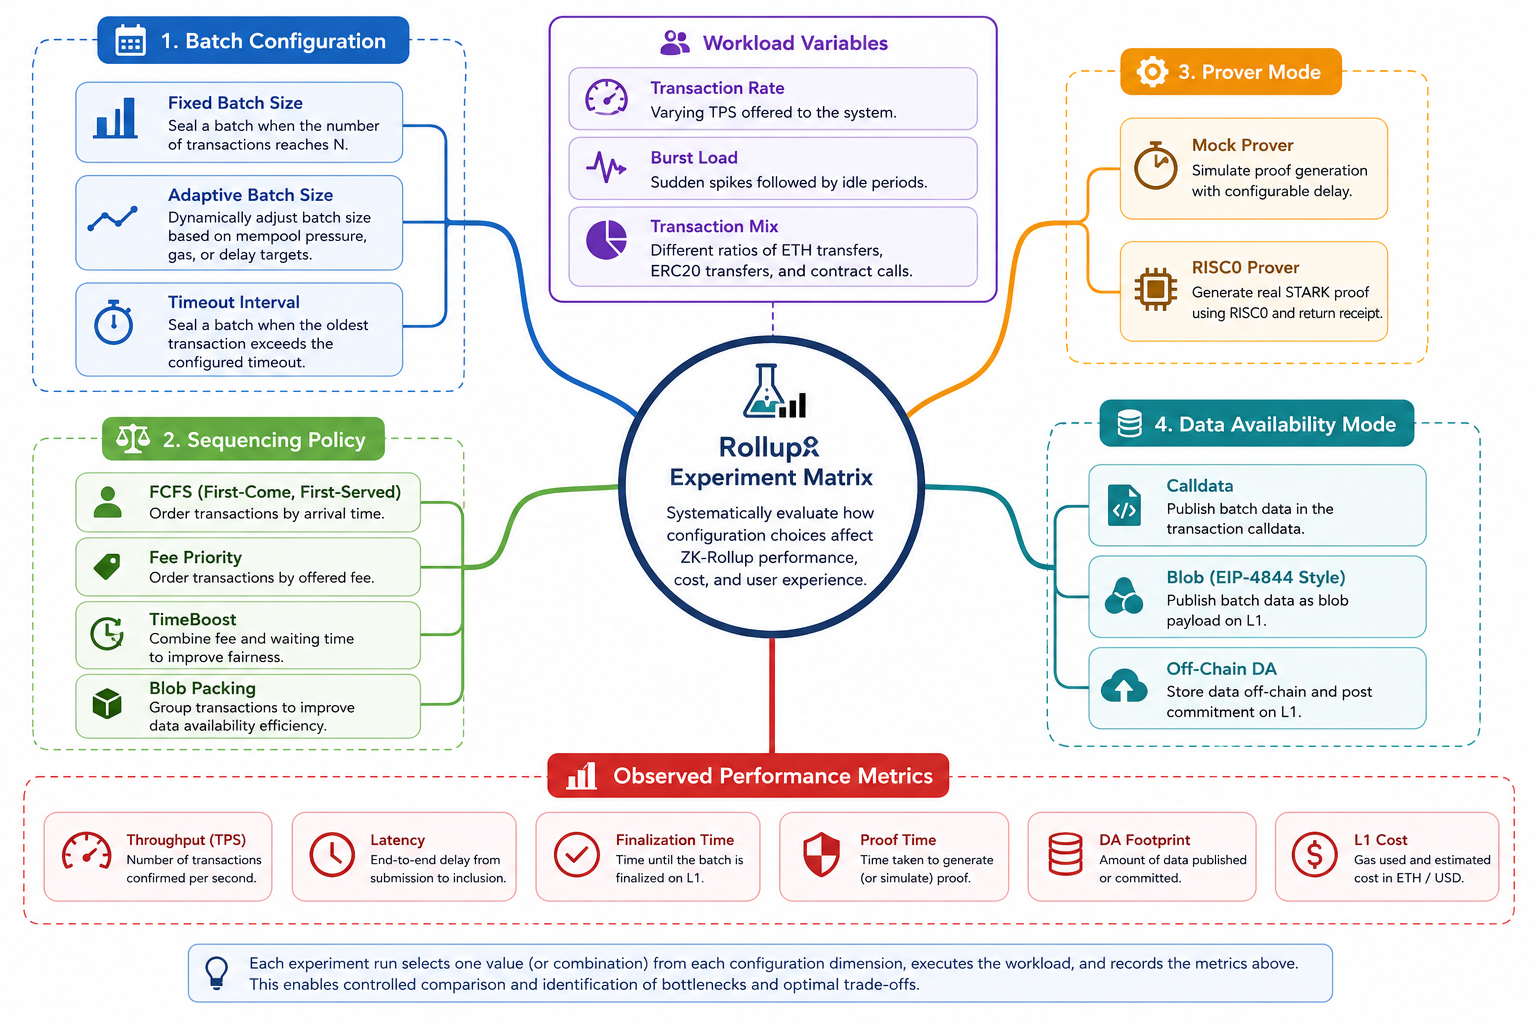
\includegraphics[
        width=0.95\textwidth,
        keepaspectratio
    ]{figures/chapter5/experiment_matrix_structure.png}
    \caption{Experiment matrix used to evaluate RollupX configuration dimensions and observed performance metrics.}
    \label{fig:experiment_matrix_structure}
\end{figure}

Figure~\ref{fig:experiment_matrix_structure} shows the main dimensions varied during the evaluation. The controlled configuration variables include batch configuration, sequencing policy, prover mode, and data availability mode. These variables represent the main design choices exposed by the RollupX framework. For example, batch configuration affects how quickly transactions are sealed into batches, sequencing policy affects ordering and fairness, prover mode affects proof-generation delay, and data availability mode affects Layer-1 publication cost.

The workload variables define the input pressure applied to the system. These include transaction rate, burst-load behaviour, and transaction mix. By changing workload characteristics separately from system configuration, the benchmark suite can evaluate both normal operating conditions and stress conditions.

The observed metrics capture the effect of each configuration on system behaviour. The evaluation records throughput, latency, finalization time, proof time, data availability footprint, and Layer-1 cost. This structure supports controlled comparison because each benchmark run can vary one primary dimension while keeping the remaining configuration stable. As a result, the analysis can identify which design choices have the strongest impact on RollupX performance and cost efficiency.

The following sections describe the testing environment, workload generation process, benchmark configurations, controlled variables, and metrics collection pipeline used to execute this experiment matrix.